\thispagestyle{empty}
\noindent
\strednp{
\NazovUniverzity\\
\NazovFakulty}
\vfill
\strednp{
\NazovDiela
%% \centerline{\PodazovDiela}
\mbox{}\\
\bigskip
\TypPrace
}
\vfill
\strednp{\textbf{\rok} \hfill{\textbf{\autor}}}
\newpage

\thispagestyle{empty}
\noindent
\strednp{\NazovUniverzity\\ \NazovFakulty}
\vfill
\strednp{\NazovDiela
%% \centerline{\PodazovDiela}
\mbox{}\\
\bigskip
\TypPrace
}
\vfill
\begin{tabular}{ l l }
\textbf{Študijný program:} & \program\\
\textbf{Študijný odbor:} & \cisloOdboru\ \odbor\\
\textbf{Školiace pracovisko:} & \katedra\\
\textbf{Vedúci práce:} &  \veduci
\end{tabular}
\bigskip\\
\bigskip\\
\bigskip\\
\bigskip\\
\strednp{\miestoRok \hfill{\autor}}
\newpage

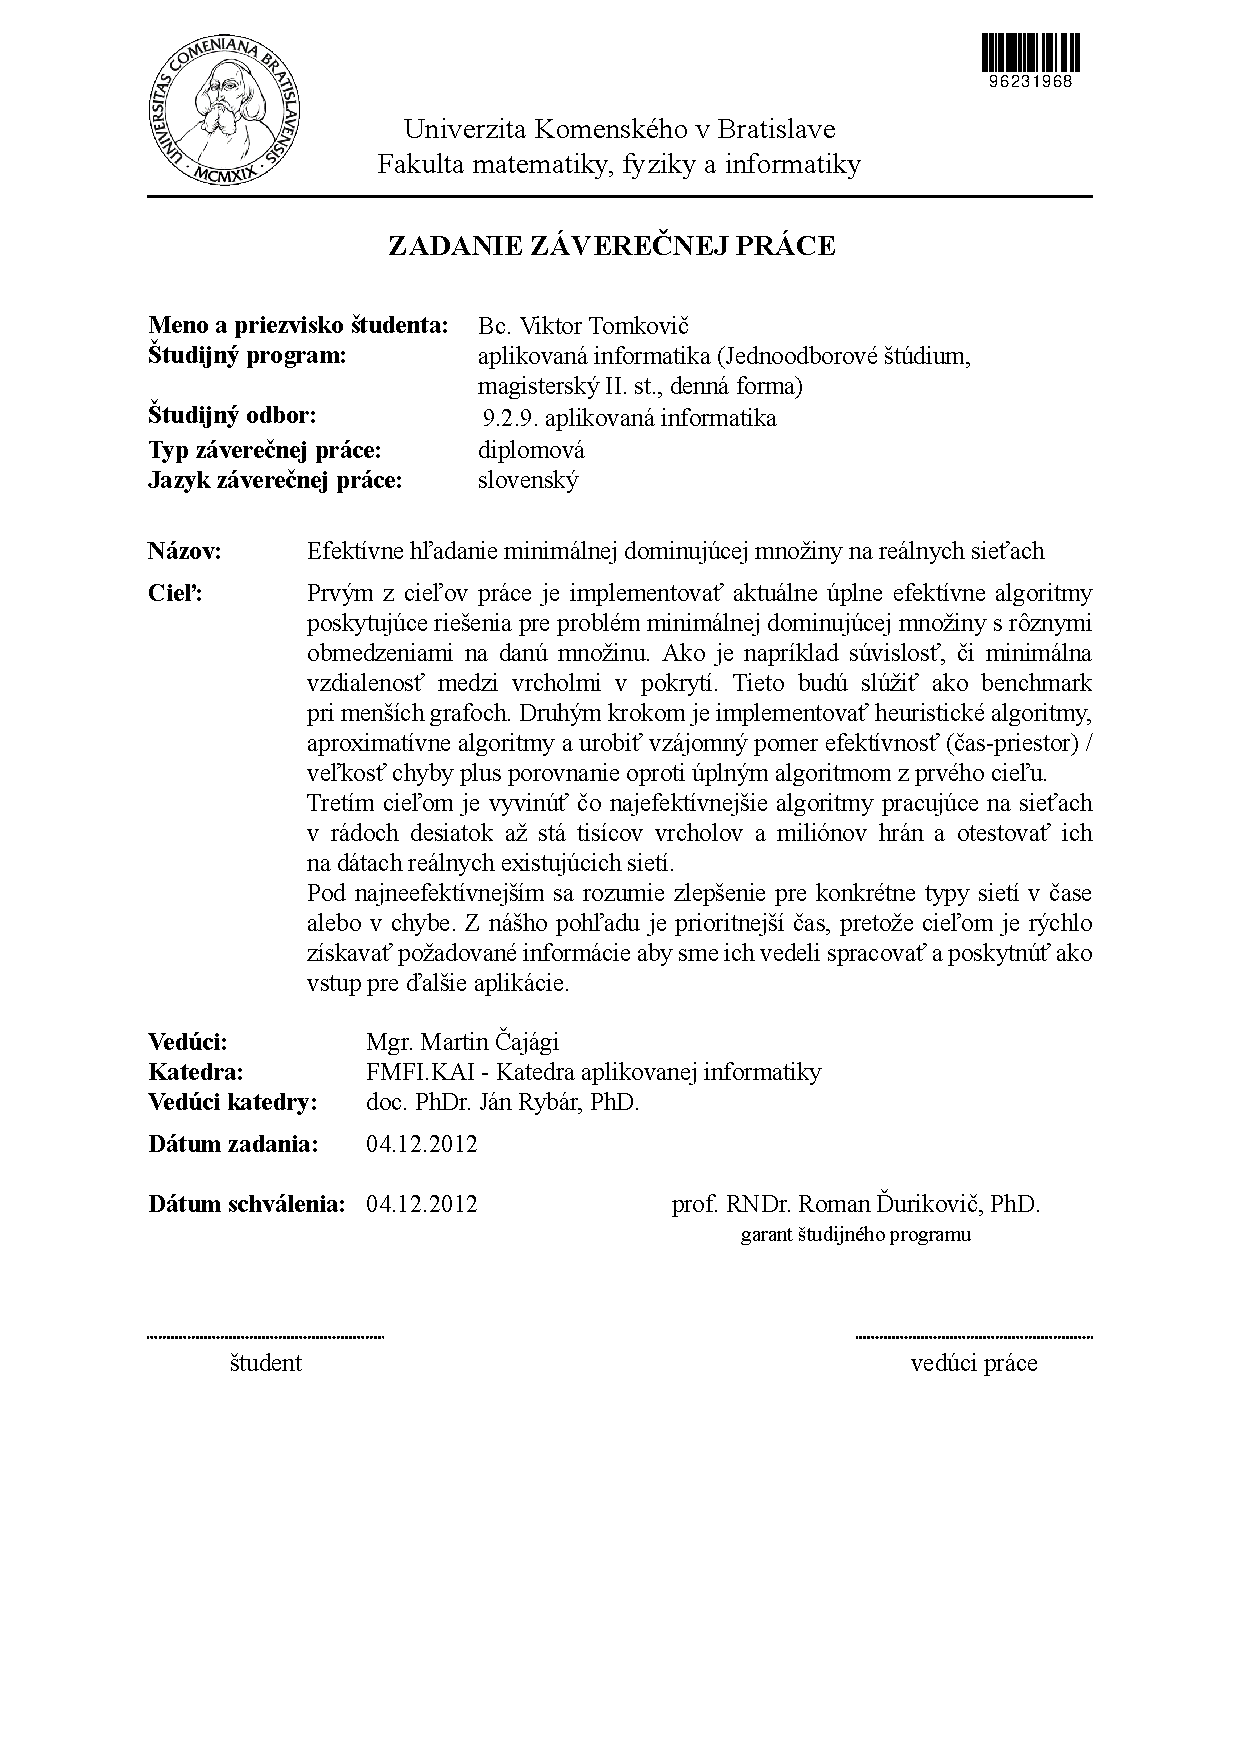
\includepdf[pages=1]{zadanie.pdf}

\newpage

\noindent
~\vfill

\section*{Poďakovanie}
Za odbornú pomoc, poskytnuté materiály a vedenie pri tejto práci patrí vďaka 
môjmu školiteľovi Martinovi Čajágimu. Taktiež by som sa chcel poďakovať 
Marekovi Zemanovi za vedenie jeho kurzom, mojim rodičom za pochopenie a 
poskytnuté možnosti vzdelávať sa a mojim priateľom za podporu.
\\
\bigskip\\
\newpage

\chapter*{Abstrakt}
Veľa reálnych sietí okolo nás má nejakú štruktúru a vlastnosti. Tieto 
vlastnosti sa snažia vedci namodelovať. Úspešne sa to darí sieťami malého 
sveta, bezškálovými sieťami a podobnými modelmi. Často sa pri práci s reálnymi 
sieťami vyskytuje problém nájdenia minimálnej dominujúcej množiny. V tejto 
práci uvádzame prehľad algoritmov na riešenie problému nájdenia minimálnej 
dominujúcej množiny. Ďalej rozoberáme algoritmy, ktoré vedú k lepšiemu 
výsledku, či už časovému alebo priestorovému, na sieťach malého sveta a 
reálnych dátach. Keďže problém je NP-úplný a reálne dáta majú príliš veľa 
vrcholov, venujeme sa najmä heuristikám pažravého algoritmu.\\
Kľúčové slová: minimálna dominujúca množina, MDS, algoritmy a dátové štruktúry, 
siete malého sveta, komplexné siete, pažravý algoritmus.

\newpage

\chapter*{Abstract}
Many real-world networks around us have some structure or features. Scientists 
try to model these features. It is successfully done with small-world networks, 
scale-free networks and with other similar networks. While working with 
small-world networks there often appears the minimum dominating set problem. 
In this work we show the state of current algorithms solving the minimum 
dominating set problem. Further on, we describe algorithms which find better 
results (considering time or set size) on small-world networks and real data. 
Because the problem is NP-complete and the size of real data is big we analyze 
heuristics of basic greedy algorithm.\\
Keywords: minimum dominating set, MDS, algorithms and date structures, small-world 
network, complex networks, greedy algorithm.
\newpage

\mbox{}
\newpage

\tableofcontents
\newpage
%\listoffigures
%\newpage
\listoftables
\newpage
